\documentclass[a4paper,12pt]{article}
\usepackage[utf8]{inputenc}
\usepackage{graphicx}
\usepackage{float}
\usepackage{listings}
\usepackage[spanish]{babel}
\usepackage{courier}
\usepackage[T1]{fontenc}

\usepackage{xcolor}
\definecolor{gris}{RGB}{123, 126, 132}
\definecolor{morado}{RGB}{81, 40, 155}
\definecolor{amarillo}{RGB}{253,151,31}
\definecolor{magenta}{RGB}{249,38,114}

\renewcommand{\lstlistingname}{Archivo}

\lstdefinestyle{customHTML}{
    frame=tb,
    language=HTML,
    backgroundcolor=\color{white},   
    commentstyle=\itshape\color{gris},
    keywordstyle=\bfseries\color{magenta},
    numberstyle=\color{morado},
    stringstyle=\color{amarillo},
    identifierstyle=\color{black},
    basicstyle=\footnotesize,
    breakatwhitespace=false,         
    breaklines=true,                 
    captionpos=b,
    keepspaces=true,                 
    numbers=left,                    
    numbersep=5pt,                  
    showspaces=false,                
    showstringspaces=false,
    showtabs=false,                  
    tabsize=2,
}

\lstdefinestyle{customJava}{
    frame=tb,
    language=Java,
    backgroundcolor=\color{white},   
    commentstyle=\itshape\color{gris},
    keywordstyle=\bfseries\color{magenta},
    numberstyle=\color{morado},
    stringstyle=\color{amarillo},
    identifierstyle=\color{black},
    basicstyle=\footnotesize,
    breakatwhitespace=false,         
    breaklines=true,                 
    captionpos=b,
    keepspaces=true,                 
    numbers=left,                    
    numbersep=5pt,                  
    showspaces=false,                
    showstringspaces=false,
    showtabs=false,                  
    tabsize=2,
}

%opening
\title{Ejercicio No. 3. Ejercicio Web Servlets JDBC}
\author{Barrera Pérez Carlos Tonatihu \\ Profesor: José Asunción Enríquez 
Zárate \\ Web Application Development \\ Grupo: 3CM9 }

\begin{document}

\maketitle
\newpage
\tableofcontents
\newpage

\section{Introducción}
Este ejercicio consistió en desarrollar una aplicación web que tuviera altas, 
bajas, cambios y consultas de carreras. La estructura de la base de datos es la 
misma que se trabajo en el ejercicio 2.

\section{Desarrollo}
Debido a que el código de DTO, DAO y de conexión a la base de datos es el mismo 
se omitirán estos archivos en el reporte, sin embargo se enviaran junto al 
reporte y el archivo war de este ejercicio.

Ahora, los siguientes archivos fueron los servlets que se utilizaron para 
controlar la funcionalidad de la aplicación, debido a que solo se utilizaron 
servlets y un HTML las vistas de las paginas web son escritas directamente por 
dichos servlets a pesar de que esto no es la mejor idea.

El siguiente archivo es el que crea el formulario para dar de alta una carrera.

\begin{lstlisting}[language=HTML, style=customHTML, 
caption={index.html}, captionpos=b, basicstyle=\fontfamily{cmss}\small]
<!DOCTYPE html>
<!--
To change this license header, choose License Headers in Project Properties.
To change this template file, choose Tools | Templates
and open the template in the editor.
-->
<html>
  <head lang="es">
    <title>TODO supply a title</title>
      <meta charset="UTF-8">
      <meta name="viewport" content="width=device-width, initial-scale=1.0">
  </head>
  <body>
    <h1>Datos de la carrera</h1>
    <div>
      <form action="AgregarCarrera" method="post">
        <p><label>Nombre de la carrera:</label><input type="text" name="nombre" 
required></p>
        <p><label>Descipcion de la carrera:</label><input type="text" 
name="descripcion" required></p>
        <p><label>Duracion de la carrera:</label><input type="number" 
name="duracion" required></p>
        <input hidden name="tipo" value="alta">
        <input type="submit" value="Enviar">
      </form>
    </div>
  </body>
</html>
\end{lstlisting}

Servlet para eliminar una carrera.

\begin{lstlisting}[language=Java, style=customJava, 
caption={EliminarCarrera.java}, captionpos=b, 
basicstyle=\fontfamily{cmss}\small]
/*
 * To change this license header, choose License Headers in Project Properties.
 * To change this template file, choose Tools | Templates
 * and open the template in the editor.
 */
package view;

import dao.CarreraDAO;
import dao.CarreraDAOImpl;
import dto.Carrera;
import java.io.IOException;
import java.io.PrintWriter;
import java.sql.SQLException;
import java.util.logging.Level;
import java.util.logging.Logger;
import javax.servlet.ServletException;
import javax.servlet.annotation.WebServlet;
import javax.servlet.http.HttpServlet;
import javax.servlet.http.HttpServletRequest;
import javax.servlet.http.HttpServletResponse;

/**
 *
 * @author tonatihu
 */
@WebServlet(name = "EliminarCarrera", urlPatterns = {"/EliminarCarrera"})
public class EliminarCarrera extends HttpServlet {

    /**
     * Processes requests for both HTTP <code>GET</code> and <code>POST</code>
     * methods.
     *
     * @param request servlet request
     * @param response servlet response
     * @throws ServletException if a servlet-specific error occurs
     * @throws IOException if an I/O error occurs
     */
    protected void processRequest(HttpServletRequest request, 
HttpServletResponse response)
            throws ServletException, IOException {
        response.setContentType("text/html;charset=UTF-8");
        try (PrintWriter out = response.getWriter()) {
            /* TODO output your page here. You may use following sample code. */
            out.println("<!DOCTYPE html>");
            out.println("<html>");
            out.println("<head>");
            out.println("<title>Servlet EliminarCarrera</title>");
            out.println("</head>");
            out.println("<body>");

            String mensajeAMostrar = "";
            Carrera c = new Carrera();
            c.setId(Integer.parseInt(request.getParameter("id")));

            CarreraDAO dao = new CarreraDAOImpl();
            try {
                dao.delete(c);
                mensajeAMostrar = "El Registro se elimino satisfactoriamente";
            } catch (SQLException ex) {
                mensajeAMostrar = "No se pudo eliminar el registro" + 
ex.toString();
                
Logger.getLogger(EliminarCarrera.class.getName()).log(Level.SEVERE, null, ex);
            }

            out.println("<div align='center'>");
            out.println(mensajeAMostrar + "<br/><br/>");
            out.println("<a href='MostrarCarrera'> Lista de Carreras </a>");
            out.println("</div>");

            out.println("</body>");
            out.println("</html>");
        }
    }

    // <editor-fold defaultstate="collapsed" desc="HttpServlet methods. 
    // Click on the + sign on the left to edit the code.">
    /**
     * Handles the HTTP <code>GET</code> method.
     *
     * @param request servlet request
     * @param response servlet response
     * @throws ServletException if a servlet-specific error occurs
     * @throws IOException if an I/O error occurs
     */
    @Override
    protected void doGet(HttpServletRequest request, HttpServletResponse 
response)
            throws ServletException, IOException {
        processRequest(request, response);
    }

    /**
     * Handles the HTTP <code>POST</code> method.
     *
     * @param request servlet request
     * @param response servlet response
     * @throws ServletException if a servlet-specific error occurs
     * @throws IOException if an I/O error occurs
     */
    @Override
    protected void doPost(HttpServletRequest request, HttpServletResponse 
response)
            throws ServletException, IOException {
        processRequest(request, response);
    }

    /**
     * Returns a short description of the servlet.
     *
     * @return a String containing servlet description
     */
    @Override
    public String getServletInfo() {
        return "Short description";
    }// </editor-fold>

}
\end{lstlisting}

Servlet para agregar carreras.

\begin{lstlisting}[language=Java, style=customJava, 
caption={AgregarCarrera.java},captionpos=b,basicstyle=\fontfamily{cmss}\small]
/*
 * To change this license header, choose License Headers in Project Properties.
 * To change this template file, choose Tools | Templates
 * and open the template in the editor.
 */
package view;

import dao.CarreraDAO;
import dao.CarreraDAOImpl;
import dto.Carrera;
import java.io.IOException;
import java.io.PrintWriter;
import java.sql.SQLException;
import java.util.logging.Level;
import java.util.logging.Logger;
import javax.servlet.ServletException;
import javax.servlet.annotation.WebServlet;
import javax.servlet.http.HttpServlet;
import javax.servlet.http.HttpServletRequest;
import javax.servlet.http.HttpServletResponse;

/**
 *
 * @author tonatihu
 */
@WebServlet(name = "AgregarCarrera", urlPatterns = {"/AgregarCarrera"})
public class AgregarCarrera extends HttpServlet {

    /**
     * Processes requests for both HTTP <code>GET</code> and <code>POST</code>
     * methods.
     *
     * @param request servlet request
     * @param response servlet response
     * @throws ServletException if a servlet-specific error occurs
     * @throws IOException if an I/O error occurs
     */
    protected void processRequest(HttpServletRequest request, 
HttpServletResponse response)
            throws ServletException, IOException {
        response.setContentType("text/html;charset=UTF-8");
        try (PrintWriter out = response.getWriter()) {
            /* TODO output your page here. You may use following sample code. */
            out.println("<!DOCTYPE html>");
            out.println("<html>");
            out.println("<head>");
            out.println("<title>Servlet AgregarAlumno</title>");
            out.println("</head>");
            out.println("<body>");
            String mensajeAMostrar = "";
            String nombreCarrera = request.getParameter("nombre");
            String descripcion = request.getParameter("descripcion");
            String tipo = request.getParameter("tipo");
            System.out.println(tipo);
            Carrera c = new Carrera();
            c.setNombre(nombreCarrera);
            c.setDescripcion(descripcion);
            c.setDuracion(Integer.parseInt(request.getParameter("duracion")));
            CarreraDAO dao = new CarreraDAOImpl();
            
            try {
                if (tipo.equals("alta")) {
                    dao.create(c);
                    mensajeAMostrar = "El Registro se agrego 
satisfactoriamente";
                } else {
                    c.setId(Integer.parseInt(request.getParameter("id")));
                    dao.update(c);
                    mensajeAMostrar = "El regustro se actualizo 
satisfactoriamente";
                }
            } catch (SQLException ex) {
                mensajeAMostrar = "No se pudo agregar el registro" + 
ex.toString();
                
Logger.getLogger(AgregarCarrera.class.getName()).log(Level.SEVERE, null, ex);
            }

            out.println("<div align='center'>");
            out.println( mensajeAMostrar +"<br/><br/>");
            out.println("<a href='MostrarCarrera'> Lista de Carreras </a>");
            out.println("</div>");

            out.println("</body>");
            out.println("</html>");
        }
    }

    // <editor-fold defaultstate="collapsed" desc="HttpServlet methods. 
    // Click on the + sign on the left to edit the code.">
    /**
     * Handles the HTTP <code>GET</code> method.
     *
     * @param request servlet request
     * @param response servlet response
     * @throws ServletException if a servlet-specific error occurs
     * @throws IOException if an I/O error occurs
     */
    @Override
    protected void doGet(HttpServletRequest request, HttpServletResponse 
response)
            throws ServletException, IOException {
        processRequest(request, response);
    }

    /**
     * Handles the HTTP <code>POST</code> method.
     *
     * @param request servlet request
     * @param response servlet response
     * @throws ServletException if a servlet-specific error occurs
     * @throws IOException if an I/O error occurs
     */
    @Override
    protected void doPost(HttpServletRequest request, HttpServletResponse 
response)
            throws ServletException, IOException {
        processRequest(request, response);
    }

    /**
     * Returns a short description of the servlet.
     *
     * @return a String containing servlet description
     */
    @Override
    public String getServletInfo() {
        return "Short description";
    }// </editor-fold>

}
\end{lstlisting}

Servlet para editar carrera.

\begin{lstlisting}[language=Java, style=customJava, 
caption={EditarCarrera.java},captionpos=b,basicstyle=\fontfamily{cmss}\small]
/*
 * To change this license header, choose License Headers in Project Properties.
 * To change this template file, choose Tools | Templates
 * and open the template in the editor.
 */
package view;

import dao.CarreraDAO;
import dao.CarreraDAOImpl;
import dto.Carrera;
import java.io.IOException;
import java.io.PrintWriter;
import java.sql.SQLException;
import java.util.logging.Level;
import java.util.logging.Logger;
import javax.servlet.ServletException;
import javax.servlet.annotation.WebServlet;
import javax.servlet.http.HttpServlet;
import javax.servlet.http.HttpServletRequest;
import javax.servlet.http.HttpServletResponse;

/**
 *
 * @author tonatihu
 */
@WebServlet(name = "EditarCarrera", urlPatterns = {"/EditarCarrera"})
public class EditarCarrera extends HttpServlet {

    /**
     * Processes requests for both HTTP <code>GET</code> and <code>POST</code>
     * methods.
     *
     * @param request servlet request
     * @param response servlet response
     * @throws ServletException if a servlet-specific error occurs
     * @throws IOException if an I/O error occurs
     */
    protected void processRequest(HttpServletRequest request, 
HttpServletResponse response)
            throws ServletException, IOException {
        response.setContentType("text/html;charset=UTF-8");
        try (PrintWriter out = response.getWriter()) {
            /* TODO output your page here. You may use following sample code. */
            CarreraDAO dao = new CarreraDAOImpl();
            Carrera carrera = new Carrera();
            carrera.setId(Integer.parseInt(request.getParameter("id")));
            try {
                carrera = dao.read(carrera);
            } catch (SQLException ex) {
                Logger.getLogger(VerCarrera.class.getName()).log(Level.SEVERE, 
null, ex);
            }
            out.println("<!DOCTYPE html>");
            out.println("<html>");
            out.println("<head>");
            out.println("<title>Servlet EditarCarrera</title>");            
            out.println("</head>");
            out.println("<body>");
            out.println("<h1>EditarCarrera</h1>");
            out.println("<form action=\"AgregarCarrera\" method=\"post\">");
            out.println("<p><label>Nombre de la carrera:</label><input 
type=\"text\" name=\"nombre\" value='" + carrera.getNombre()+ "'></p>");
            out.println("<p><label>Descipcion de la carrera:</label><input 
type=\"text\" name=\"descripcion\" value='" + carrera.getDescripcion()+ 
"'></p>");
            out.println("<p><label>Duracion de la carrera:</label><input 
type=\"number\" name=\"duracion\" value='" + carrera.getDuracion()+ "'></p>");
            out.println("<input hidden name=\"tipo\" value=\"cambio\">");
            out.println("<input hidden name=\"id\" value='" + carrera.getId() 
+"'>");
            out.println("<input type=\"submit\" value=\"Enviar\">");
            out.println("</form>");
            out.println("</body>");
            out.println("</html>");
        }
    }

    // <editor-fold defaultstate="collapsed" desc="HttpServlet methods. 
    // Click on the + sign on the left to edit the code.">
    /**
     * Handles the HTTP <code>GET</code> method.
     *
     * @param request servlet request
     * @param response servlet response
     * @throws ServletException if a servlet-specific error occurs
     * @throws IOException if an I/O error occurs
     */
    @Override
    protected void doGet(HttpServletRequest request, HttpServletResponse 
response)
            throws ServletException, IOException {
        processRequest(request, response);
    }

    /**
     * Handles the HTTP <code>POST</code> method.
     *
     * @param request servlet request
     * @param response servlet response
     * @throws ServletException if a servlet-specific error occurs
     * @throws IOException if an I/O error occurs
     */
    @Override
    protected void doPost(HttpServletRequest request, HttpServletResponse 
response)
            throws ServletException, IOException {
        processRequest(request, response);
    }

    /**
     * Returns a short description of the servlet.
     *
     * @return a String containing servlet description
     */
    @Override
    public String getServletInfo() {
        return "Short description";
    }// </editor-fold>

}

\end{lstlisting}

Servlet para mostrar varias carreras.

\begin{lstlisting}[language=Java, style=customJava, 
caption={VerCarrera.java},captionpos=b,basicstyle=\fontfamily{cmss}\small]
/*
 * To change this license header, choose License Headers in Project Properties.
 * To change this template file, choose Tools | Templates
 * and open the template in the editor.
 */
package view;

import dao.CarreraDAO;
import dao.CarreraDAOImpl;
import dto.Carrera;
import java.io.IOException;
import java.io.PrintWriter;
import java.sql.SQLException;
import java.util.logging.Level;
import java.util.logging.Logger;
import javax.servlet.ServletException;
import javax.servlet.annotation.WebServlet;
import javax.servlet.http.HttpServlet;
import javax.servlet.http.HttpServletRequest;
import javax.servlet.http.HttpServletResponse;

/**
 *
 * @author tonatihu
 */
@WebServlet(name = "VerCarrera", urlPatterns = {"/VerCarrera"})
public class VerCarrera extends HttpServlet {

    /**
     * Processes requests for both HTTP <code>GET</code> and <code>POST</code>
     * methods.
     *
     * @param request servlet request
     * @param response servlet response
     * @throws ServletException if a servlet-specific error occurs
     * @throws IOException if an I/O error occurs
     */
    protected void processRequest(HttpServletRequest request, 
HttpServletResponse response)
            throws ServletException, IOException {
        response.setContentType("text/html;charset=UTF-8");
        try (PrintWriter out = response.getWriter()) {
            /* TODO output your page here. You may use following sample code. */
            out.println("<!DOCTYPE html>");
            out.println("<html>");
            out.println("<head>");
            out.println("<title>Servlet VerCarrera</title>");
            out.println("</head>");
            out.println("<body>");

            out.println("<h3 align='center'>Datos de la Carrera</h3>");
            out.println("<table align='center' border='1' width='60%'");
            CarreraDAO dao = new CarreraDAOImpl();
            Carrera carrera = new Carrera();
            carrera.setId(Integer.parseInt(request.getParameter("id")));
            try {
                carrera = dao.read(carrera);
            } catch (SQLException ex) {
                Logger.getLogger(VerCarrera.class.getName()).log(Level.SEVERE, 
null, ex);
            }
            if (carrera != null) {
            out.println("<tr>");
            out.println("<th> Id Carrera </th><td>" + carrera.getId() + 
"</td>");
            out.println("</tr>");
            out.println("<tr>");
            out.println("<th> Nombre Carrera </th><td>" + carrera.getNombre() + 
"</td>");
            out.println("</tr>");
            out.println("<tr>");
            out.println("<th> Descripci&oacute;n Carrera </th><td>" + 
carrera.getDescripcion() + "</td>");
            out.println("</tr>");
            out.println("<tr>");
            out.println("<th> Duraci&oacute;n Carrera </th><td>" + 
carrera.getDuracion() + "</td>");
            out.println("</tr>");
            out.println("</table>");
            out.println("<div align='center'>");
            out.println("<a href='EliminarCarrera?id=" + carrera.getId() +" '> 
Eliminar Carrera </a>");
            out.println("&nbsp; &nbsp; &nbsp;");
            out.println("<a href='MostrarCarrera'> Lista de Carreras </a>");
            out.println("</div>");
            }

            out.println("</body>");
            out.println("</html>");
        }
    }

    // <editor-fold defaultstate="collapsed" desc="HttpServlet methods. 
    // Click onthe + sign on the left to edit the code.">
    /**
     * Handles the HTTP <code>GET</code> method.
     *
     * @param request servlet request
     * @param response servlet response
     * @throws ServletException if a servlet-specific error occurs
     * @throws IOException if an I/O error occurs
     */
    @Override
    protected void doGet(HttpServletRequest request, HttpServletResponse 
response)
            throws ServletException, IOException {
        processRequest(request, response);
    }

    /**
     * Handles the HTTP <code>POST</code> method.
     *
     * @param request servlet request
     * @param response servlet response
     * @throws ServletException if a servlet-specific error occurs
     * @throws IOException if an I/O error occurs
     */
    @Override
    protected void doPost(HttpServletRequest request, HttpServletResponse 
response)
            throws ServletException, IOException {
        processRequest(request, response);
    }

    /**
     * Returns a short description of the servlet.
     *
     * @return a String containing servlet description
     */
    @Override
    public String getServletInfo() {
        return "Short description";
    }// </editor-fold>

}

\end{lstlisting}

Servlet para mostrar una carrera.

\begin{lstlisting}[language=Java, style=customJava, 
caption={MostrarCarrera.java},captionpos=b,basicstyle=\fontfamily{cmss}\small]
/*
 * To change this license header, choose License Headers in Project Properties.
 * To change this template file, choose Tools | Templates
 * and open the template in the editor.
 */
package view;

import dao.CarreraDAO;
import dao.CarreraDAOImpl;
import dto.Carrera;
import java.io.IOException;
import java.io.PrintWriter;
import java.sql.SQLException;
import java.util.List;
import java.util.logging.Level;
import java.util.logging.Logger;
import javax.servlet.ServletException;
import javax.servlet.annotation.WebServlet;
import javax.servlet.http.HttpServlet;
import javax.servlet.http.HttpServletRequest;
import javax.servlet.http.HttpServletResponse;

/**
 *
 * @author tonatihu
 */
@WebServlet(name = "MostrarCarrera", urlPatterns = {"/MostrarCarrera"})
public class MostrarCarrera extends HttpServlet {

    /**
     * Processes requests for both HTTP <code>GET</code> and <code>POST</code>
     * methods.
     *
     * @param request servlet request
     * @param response servlet response
     * @throws ServletException if a servlet-specific error occurs
     * @throws IOException if an I/O error occurs
     */
    protected void processRequest(HttpServletRequest request, 
HttpServletResponse response)
            throws ServletException, IOException {
        response.setContentType("text/html;charset=UTF-8");
        try (PrintWriter out = response.getWriter()) {
            /* TODO output your page here. You may use following sample code. */
            out.println("<!DOCTYPE html>");
            out.println("<html>");
            out.println("<head>");
            out.println("<link rel=\"stylesheet\" "
                    + 
"href=\"https://use.fontawesome.com/releases/v5.7.2/css/all.css\" "
                    + 
"integrity=\"sha384-fnmOCqbTlWIlj8LyTjo7mOUStjsKC4pOpQbqyi7RrhN7udi9RwhKkMHpvLbH
G9Sr\" "
                    + "crossorigin=\"anonymous\">");
            out.println("<title>Servlet MostrarCarrera</title>");
            out.println("</head>");
            out.println("<body>");

            String nombreCarrera, descripcionCarrera;
            String mensajeAMostrar = "";
            int idCarrera, duracionCarrera;

            out.println("<h3 align='center'>Lista de Carreras</h3>");
            out.println("<table align='center' border='1' width='60%'");
            out.println("<tr>");
            out.println("<th> Id Carrera </th>");
            out.println("<th> Nombre Carrera </th>");
            out.println("<th> Descripci&oacute;n Carrera </th>");
            out.println("<th> Duraci&oacute;n Carrera </th>");
            out.println("<th>Acciones<table><tr><td>Ver</td>"
                    + "<td>Actualizar</td><td>Eliminar</td></tr></table></th>");
            out.println("</tr>");

            CarreraDAO dao = new CarreraDAOImpl();
            try {
                List<Carrera> lista = dao.readAll();
                for (int i = 0; i < lista.size(); i++) {
                    Carrera listaCarrera = (Carrera) lista.get(i);
                    idCarrera = listaCarrera.getId();
                    nombreCarrera = listaCarrera.getNombre();
                    descripcionCarrera = listaCarrera.getDescripcion();
                    duracionCarrera = listaCarrera.getDuracion();

                    out.println("<tr>");
                    out.println("<td><a href='VerCarrera?id=" + idCarrera + "' 
>" + idCarrera + "</a></td>");
                    out.println("<td>" + nombreCarrera + "</td>");
                    out.println("<td>" + descripcionCarrera + "</td>");
                    out.println("<td>" + duracionCarrera + "</td>");
                    out.println("<td><table><tr>"
                            + "<td><a href='EliminarCarrera?id=" + idCarrera + 
"' ><i class='fas fa-trash'></i></a></td>"
                            + "<td><a href='VerCarrera?id="+idCarrera+"'><i 
class='fas fa-eye'></i></a></td>"
                            + "<td><a href='EditarCarrera?id="+idCarrera+"'><i 
class='fas fa-edit'></i></a></td>"
                            + "</tr></table></td>");
                    out.println("</tr>");
                }
                out.println("</table>");

                out.println("<div align='center'>");
                out.println("<a href='index.html'> Agregar Carrera </a>");
                out.println("</div>");
            } catch (SQLException e) {
                mensajeAMostrar = "No se pudo mostrar el listado de Carreras" + 
e.toString();
                out.println("<div align='center'>");
                out.println(mensajeAMostrar + "<br/><br/>");
                out.println("</div>");
                
Logger.getLogger(MostrarCarrera.class.getName()).log(Level.SEVERE, null, e);
            }
            out.println("</body>");
            out.println("</html>");
        }
    }

    // <editor-fold defaultstate="collapsed" desc="HttpServlet methods. 
    // Click on the + sign on the left to edit the code.">
    /**
     * Handles the HTTP <code>GET</code> method.
     *
     * @param request servlet request
     * @param response servlet response
     * @throws ServletException if a servlet-specific error occurs
     * @throws IOException if an I/O error occurs
     */
    @Override
    protected void doGet(HttpServletRequest request, HttpServletResponse 
response)
            throws ServletException, IOException {
        processRequest(request, response);
    }

    /**
     * Handles the HTTP <code>POST</code> method.
     *
     * @param request servlet request
     * @param response servlet response
     * @throws ServletException if a servlet-specific error occurs
     * @throws IOException if an I/O error occurs
     */
    @Override
    protected void doPost(HttpServletRequest request, HttpServletResponse 
response)
            throws ServletException, IOException {
        processRequest(request, response);
    }

    /**
     * Returns a short description of the servlet.
     *
     * @return a String containing servlet description
     */
    @Override
    public String getServletInfo() {
        return "Short description";
    }// </editor-fold>

}

\end{lstlisting}

Las siguientes son las pruebas que se hicieron para verificar el correcto 
funcionamiento de la aplicación.

\subsection{Eliminar}

\begin{figure}[H]
\begin{center}
 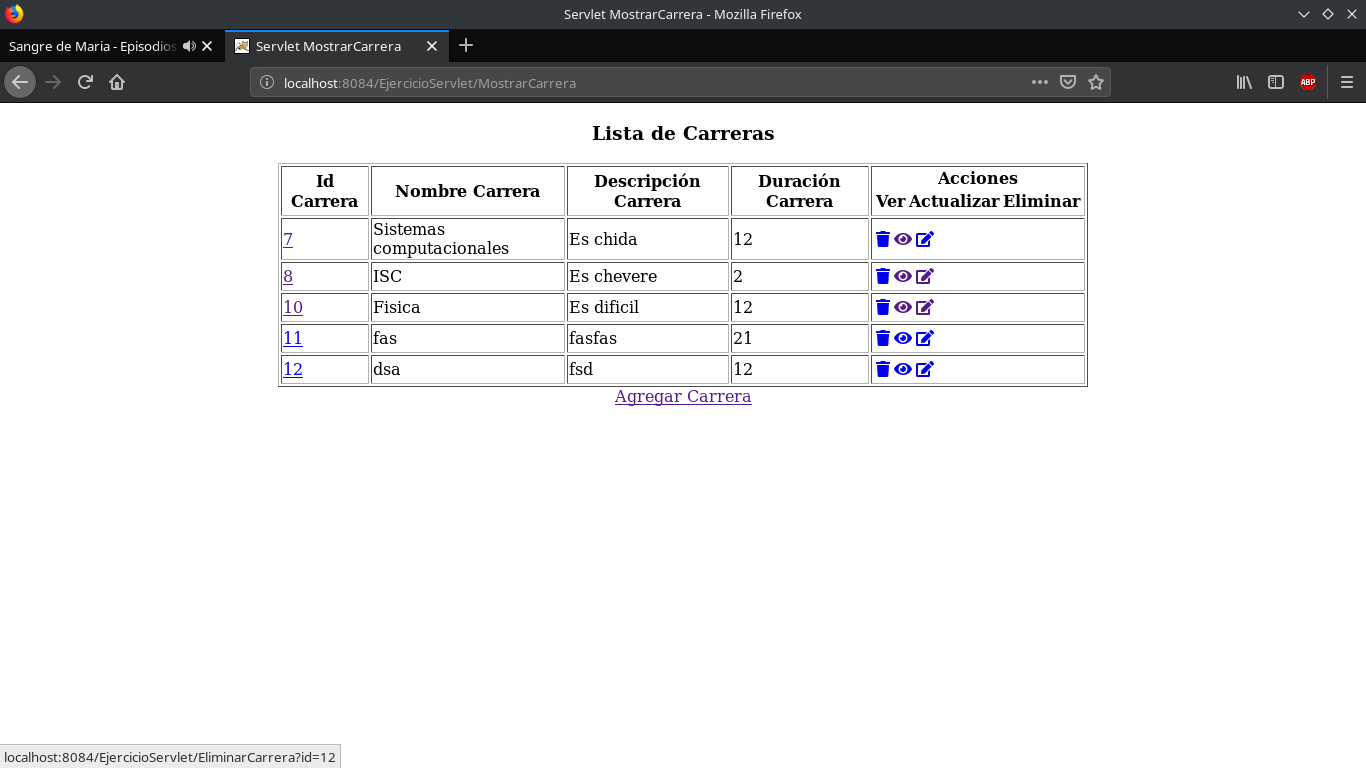
\includegraphics[width=\textwidth]{img/baja1.png}
 % estructura.png: 800x436 px, 96dpi, 21.16x11.53 cm, bb=0 0 600 327
 \caption{Se muestran todas las carreras que existen}
 \label{fig:baja1}
\end{center}
\end{figure}

\begin{figure}[H]
\begin{center}
 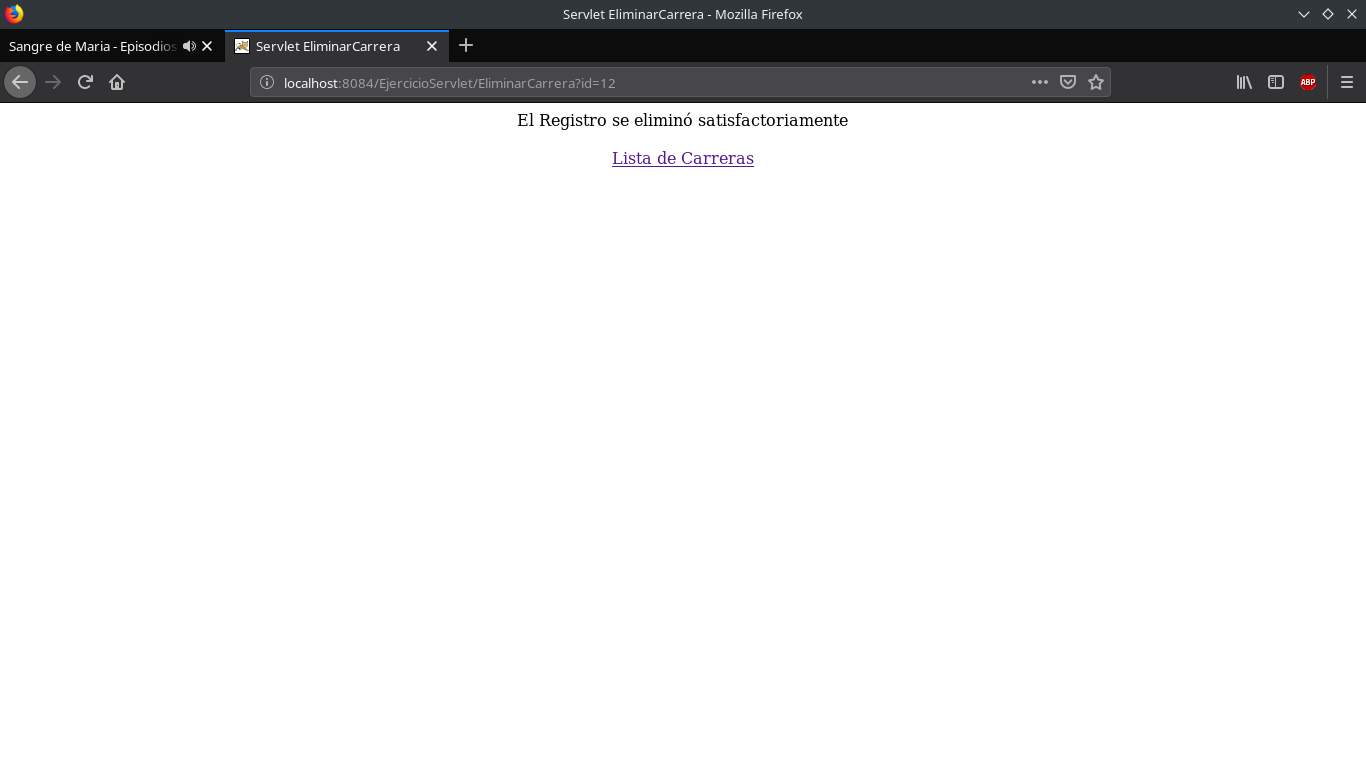
\includegraphics[width=\textwidth]{img/baja2.png}
 % estructura.png: 800x436 px, 96dpi, 21.16x11.53 cm, bb=0 0 600 327
 \caption{Después seleccionamos la ultima carrera y la eliminamos}
 \label{fig:baja2}
\end{center}
\end{figure}

\subsection{Ver}

\begin{figure}[H]
\begin{center}
 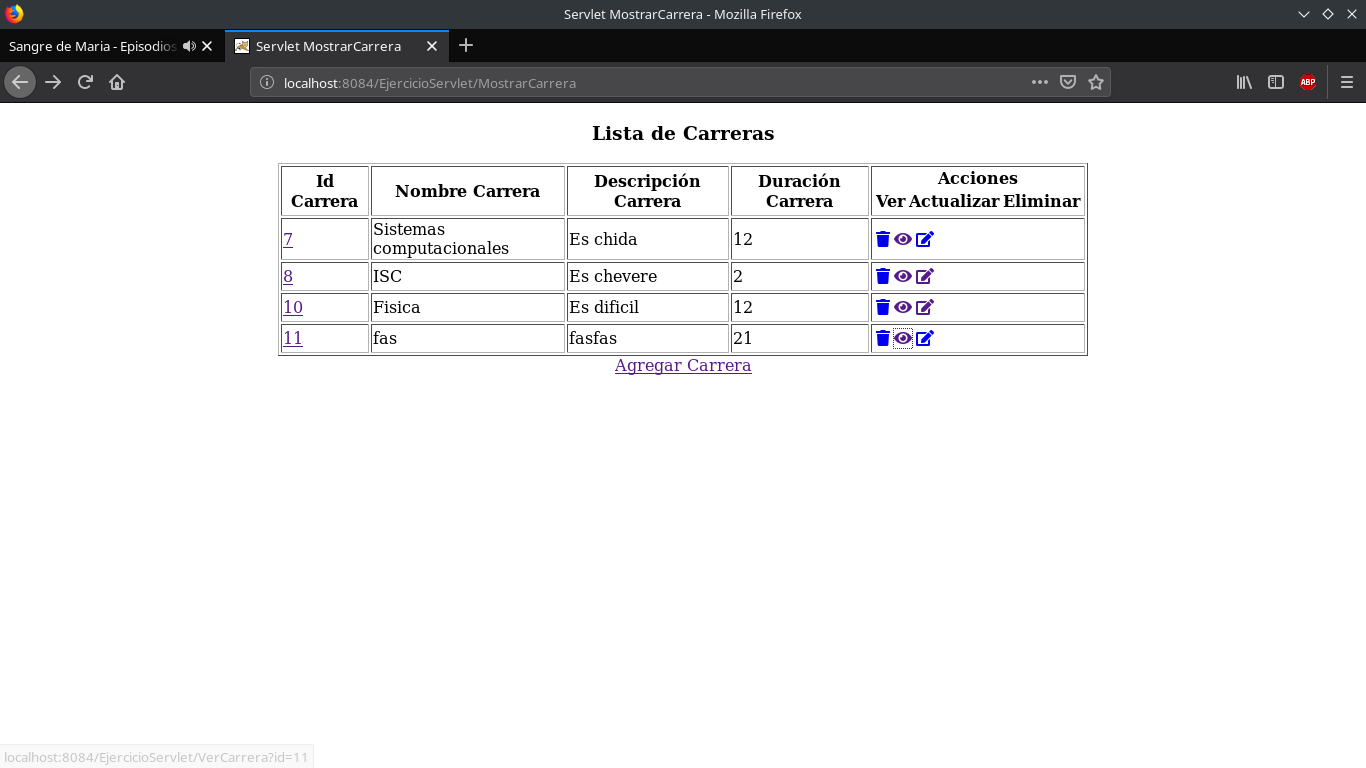
\includegraphics[width=\textwidth]{img/ver1.png}
 % estructura.png: 800x436 px, 96dpi, 21.16x11.53 cm, bb=0 0 600 327
 \caption{Se puede apreciar que se borro la carrera del paso anterior}
 \label{fig:ver1}
\end{center}
\end{figure}

\begin{figure}[H]
\begin{center}
 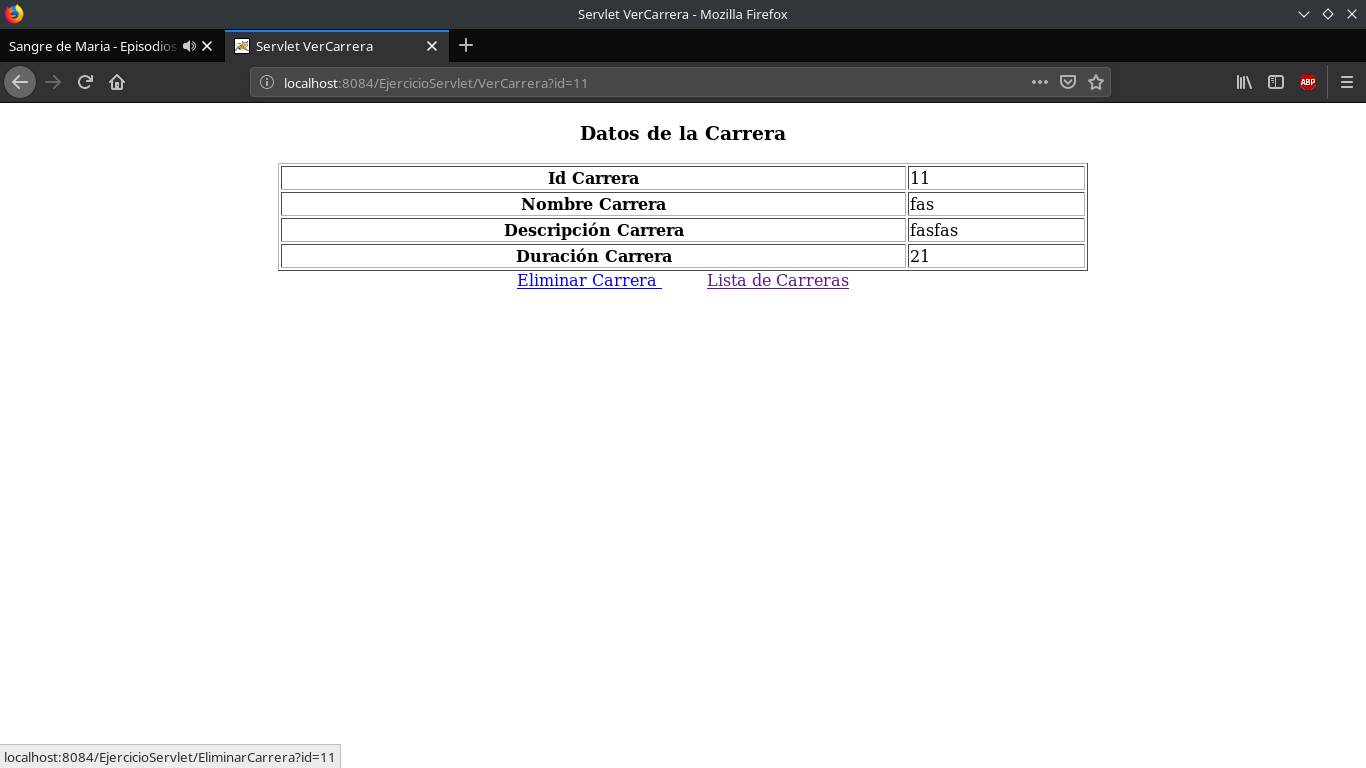
\includegraphics[width=\textwidth]{img/ver2.png}
 % estructura.png: 800x436 px, 96dpi, 21.16x11.53 cm, bb=0 0 600 327
 \caption{Al darle click en el boton de ver observamos los detalles de la 
carrera}
 \label{fig:ver2}
\end{center}
\end{figure}

\begin{figure}[H]
\begin{center}
 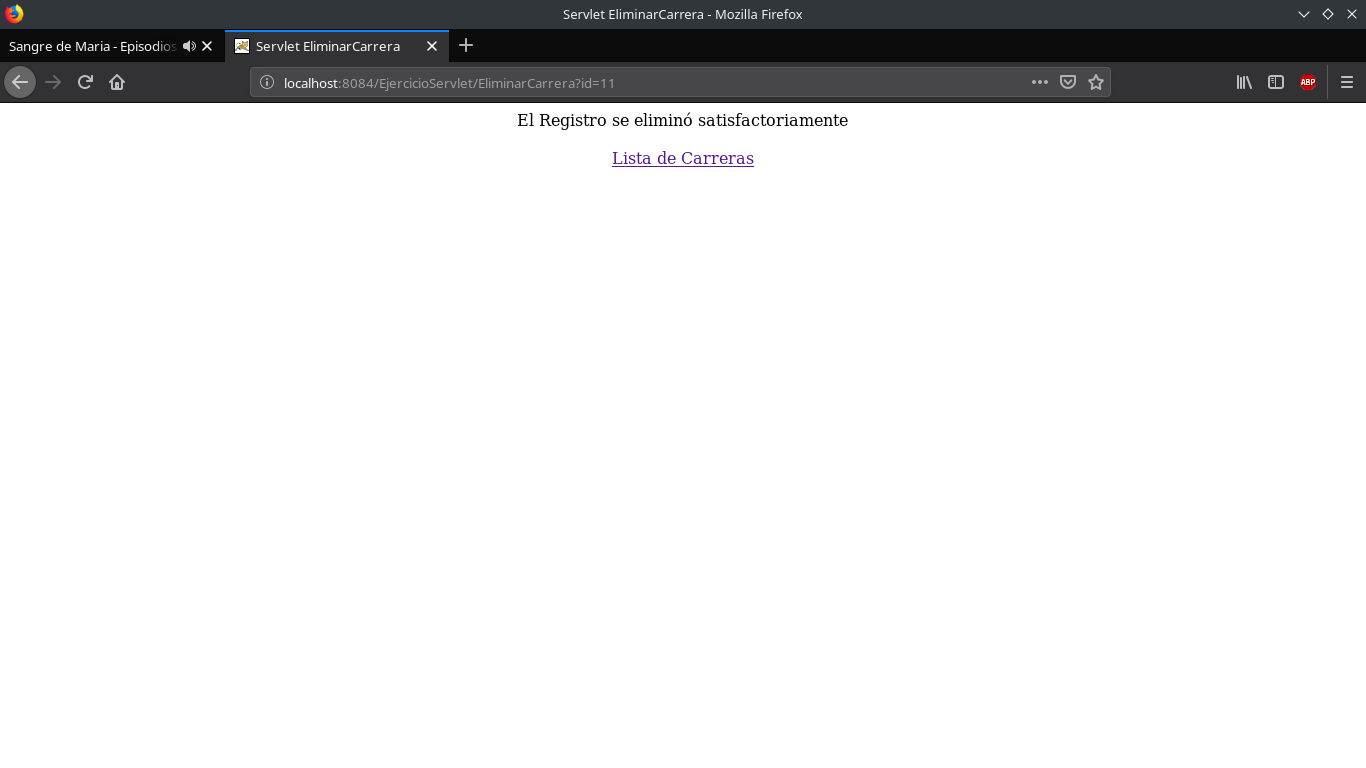
\includegraphics[width=\textwidth]{img/ver3.png}
 % estructura.png: 800x436 px, 96dpi, 21.16x11.53 cm, bb=0 0 600 327
 \caption{Damos click en eliminar carrera y se elimina}
 \label{fig:ver3}
\end{center}
\end{figure}

\subsection{Editar}

\begin{figure}[H]
\begin{center}
 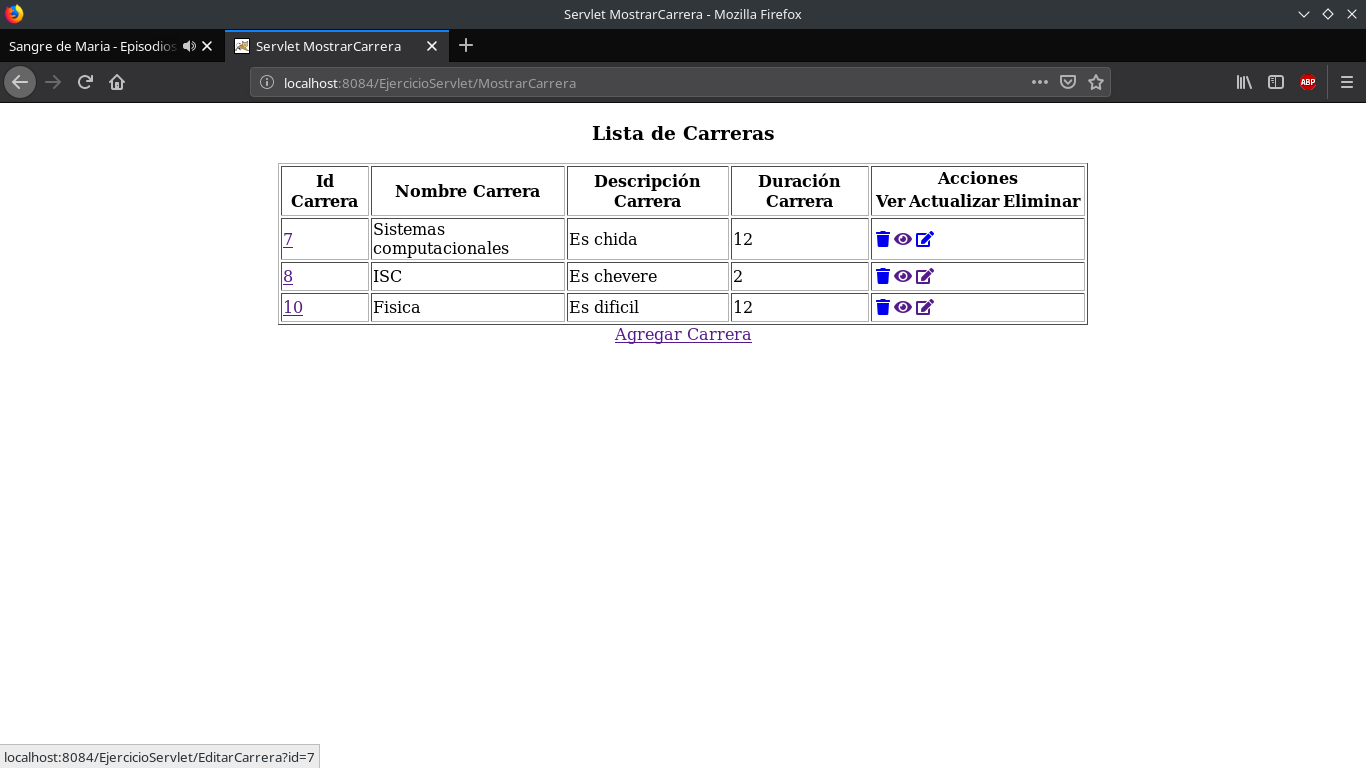
\includegraphics[width=\textwidth]{img/editar1.png}
 % estructura.png: 800x436 px, 96dpi, 21.16x11.53 cm, bb=0 0 600 327
 \caption{La carrera anterior ya no existe, ahora editaremos una}
 \label{fig:editar1}
\end{center}
\end{figure}

\begin{figure}[H]
\begin{center}
 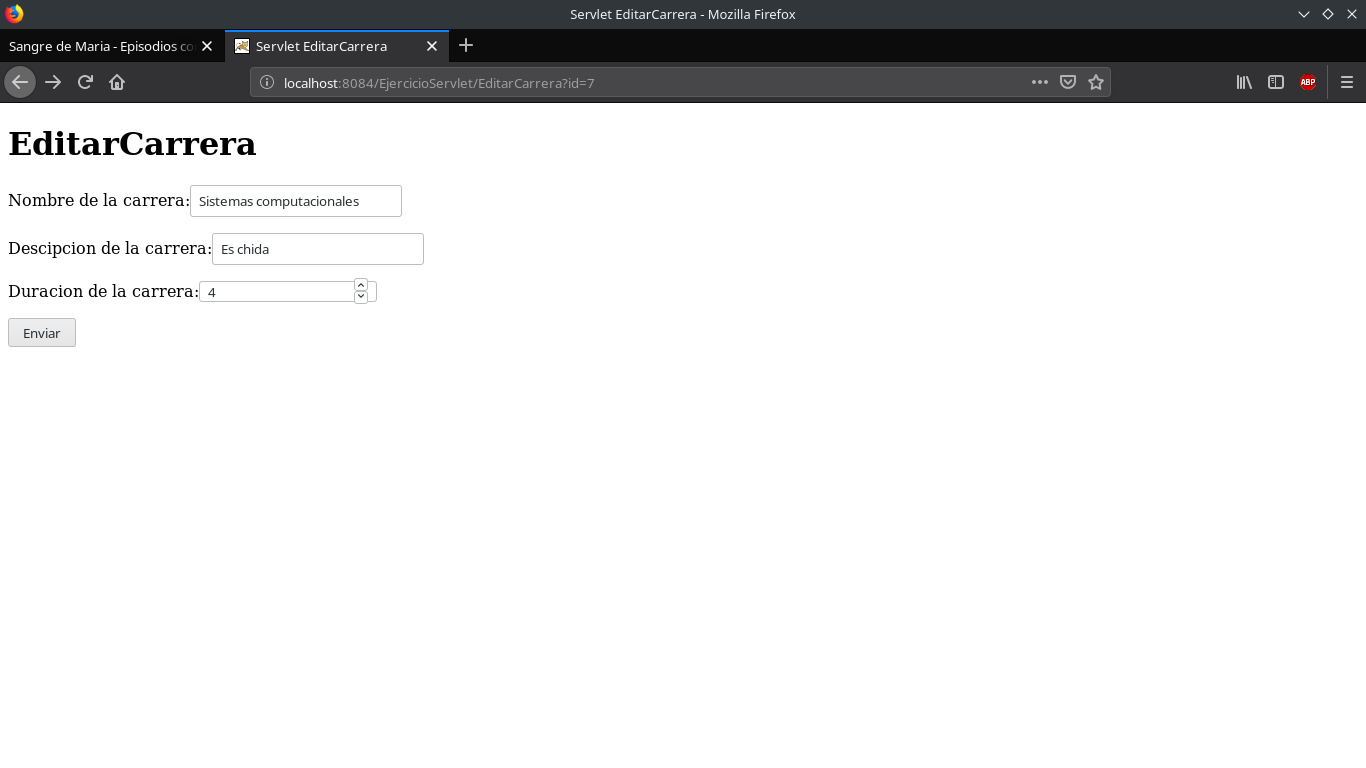
\includegraphics[width=\textwidth]{img/editar2.png}
 % estructura.png: 800x436 px, 96dpi, 21.16x11.53 cm, bb=0 0 600 327
 \caption{Aparece el formulario y cambiamos los datos}
 \label{fig:editar2}
\end{center}
\end{figure}

\begin{figure}[H]
\begin{center}
 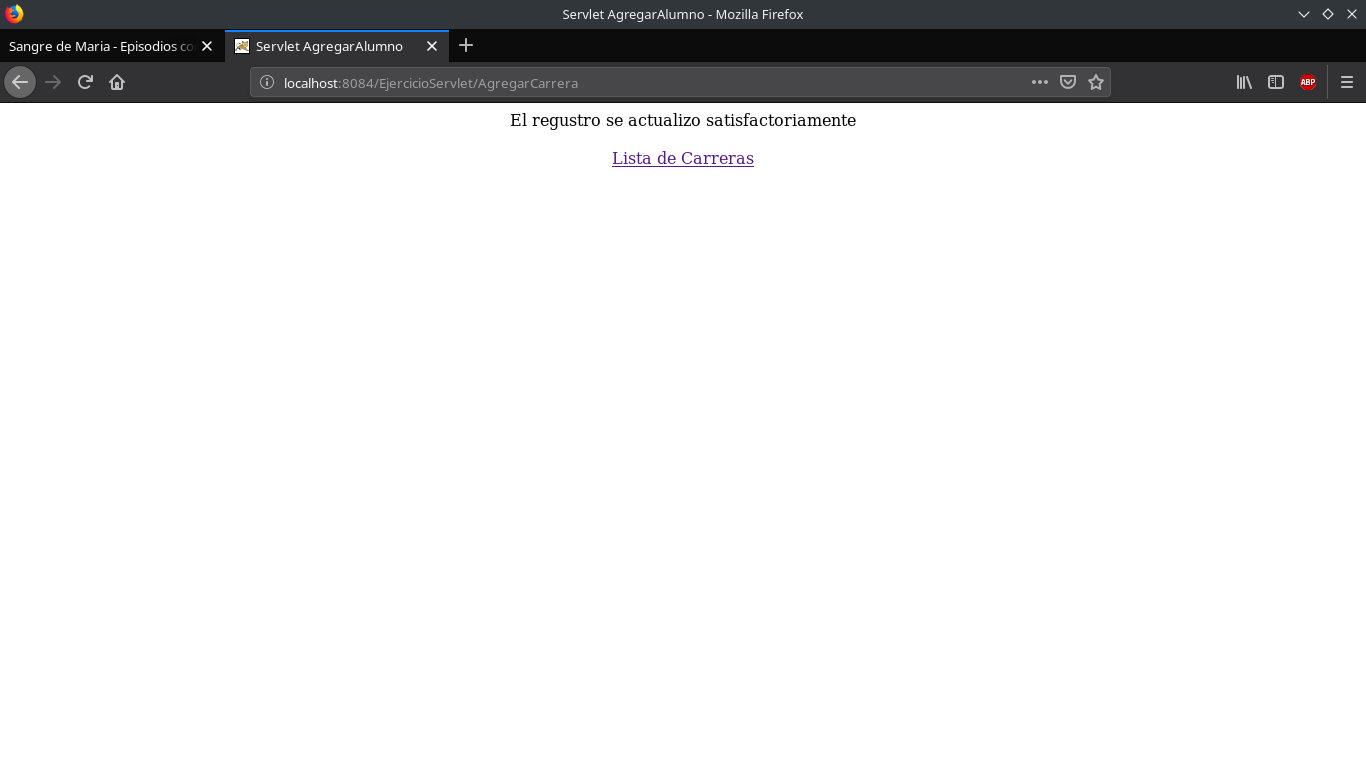
\includegraphics[width=\textwidth]{img/editar3.png}
 % estructura.png: 800x436 px, 96dpi, 21.16x11.53 cm, bb=0 0 600 327
 \caption{Nos aparece el mensaje de todo correcto}
 \label{fig:editar3}
\end{center}
\end{figure}

\subsection{Alta}

\begin{figure}[H]
\begin{center}
 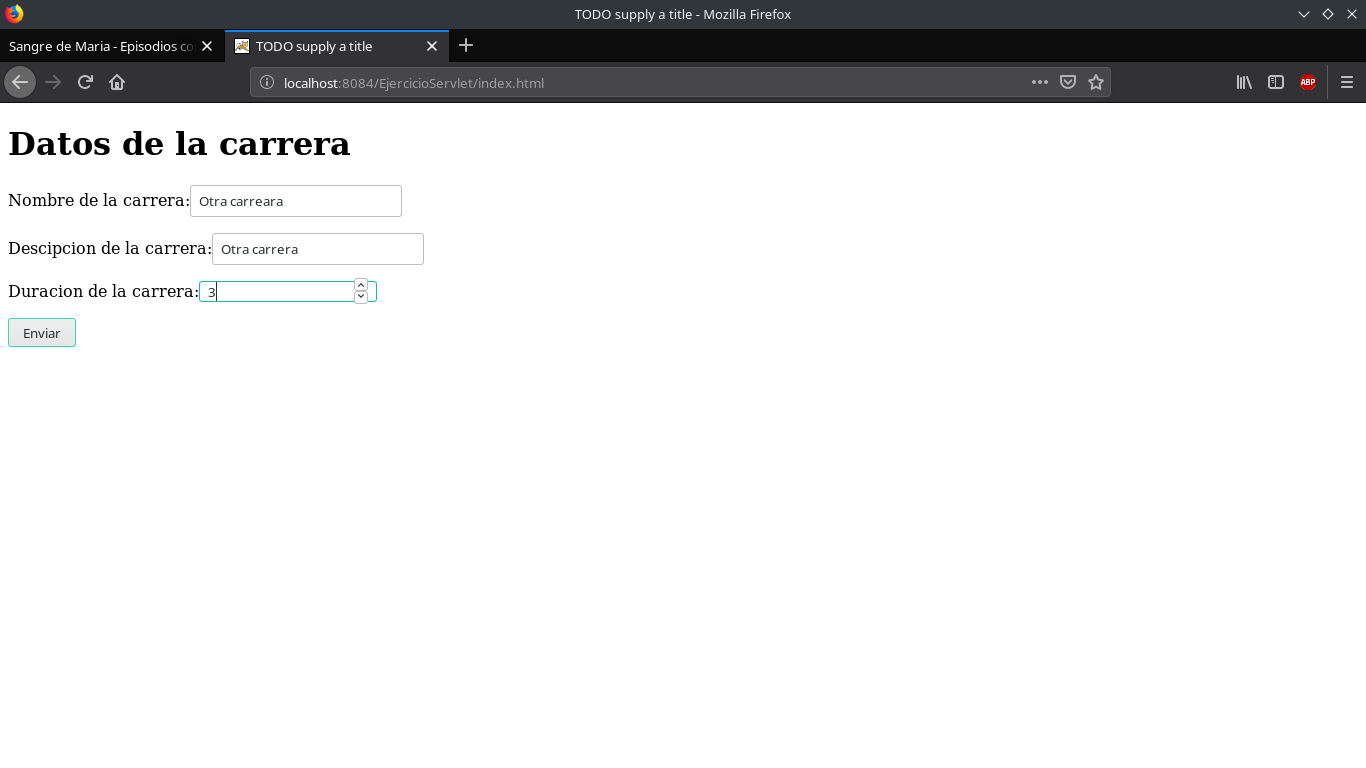
\includegraphics[width=\textwidth]{img/alta1.png}
 % estructura.png: 800x436 px, 96dpi, 21.16x11.53 cm, bb=0 0 600 327
 \caption{Creamos una carrera}
 \label{fig:alta1}
\end{center}
\end{figure}

\begin{figure}[H]
\begin{center}
 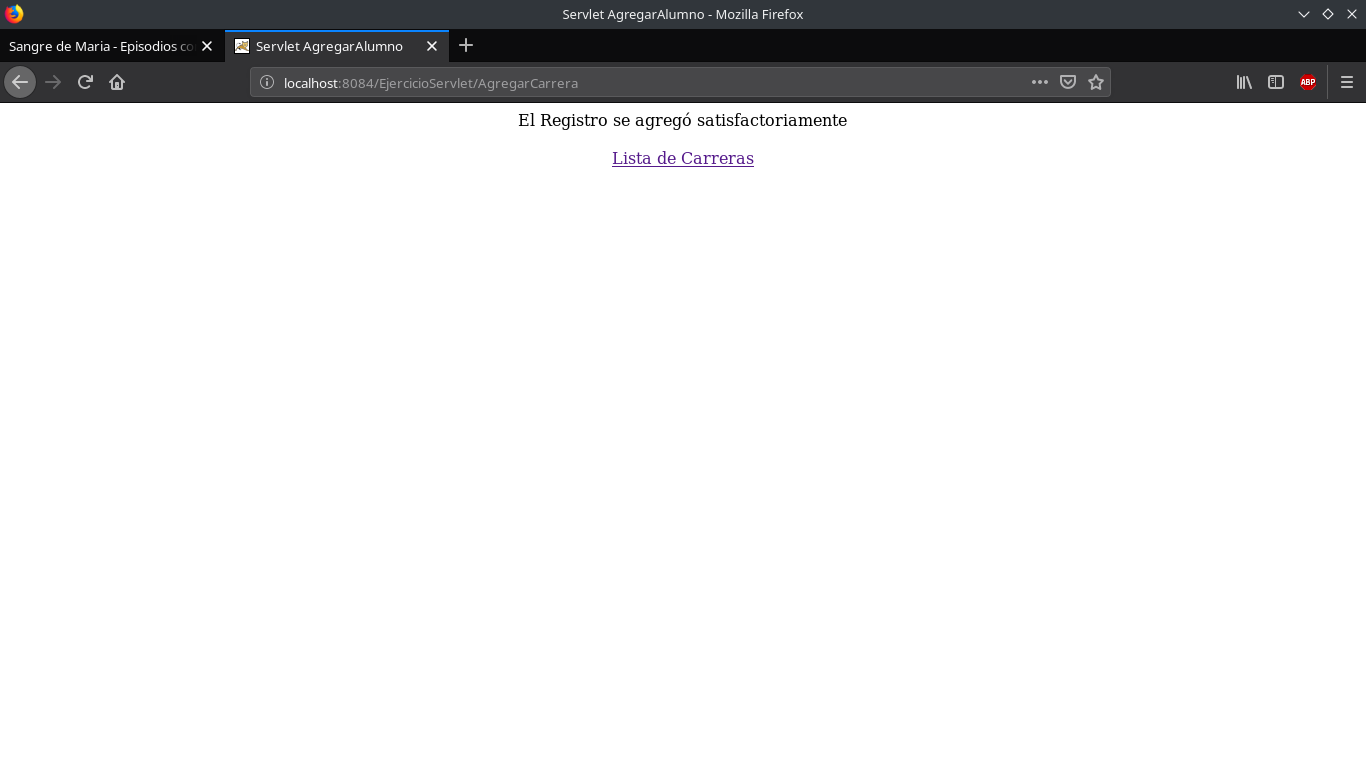
\includegraphics[width=\textwidth]{img/alta2.png}
 % estructura.png: 800x436 px, 96dpi, 21.16x11.53 cm, bb=0 0 600 327
 \caption{Pulsamos el boton del formulario y recibimos el siguiente mensaje}
 \label{fig:alta2}
\end{center}
\end{figure}

\section{Conclusiones}
Este fue un ejemplo bastante útil para entender el como funcionan los servlets 
y el como se realiza una aplicación web al dividir los componentes de dicha 
aplicación y con ello poder hacer modificaciones de ser necesario.

\end{document}
